\notechapter{N-20260305}{Orthogonal Projection, Least Squares, and the Pseudoinverse}


\section{Projection onto a subspace}

Let $U\subseteq\mathbb R^n$ have ordered basis $b_1,\ldots,b_m$ and put
\[
  B=(b_1,\ldots,b_m)\in\mathbb R^{n\times m}.
\]
The orthogonal projection of $x$ onto $U$ has the form $B\lambda$.  The error must be orthogonal to $U$:
\[
  B^T(x-B\lambda)=0.
\]
Thus
\[
  B^TB\lambda=B^Tx,\qquad \lambda=(B^TB)^{-1}B^Tx,
\]
assuming the columns of $B$ are independent.  Therefore
\[
  \boxed{\pi_U(x)=B(B^TB)^{-1}B^Tx.}
\]

\section{Projection matrix and least squares}

The matrix
\[
  P_U=B(B^TB)^{-1}B^T
\]
is symmetric and idempotent:
\[
  P_U^T=P_U,\qquad P_U^2=P_U.
\]
For an overdetermined system $B\lambda\approx x$, minimizing $\|B\lambda-x\|^2$ gives the same normal equations.  Least squares is orthogonal projection written in coordinates.

\section{Pseudoinverse}

When $B$ has full column rank, the Moore--Penrose pseudoinverse is
\[
  B^+=(B^TB)^{-1}B^T.
\]
For a general matrix $A=U\Sigma V^T$, the pseudoinverse is $A^+=V\Sigma^+U^T$, where nonzero singular values are inverted.  This makes SVD the stable language of projection and least-squares computation.


\section{Projection geometry in the source diagram}

The diagram is kept because projection and least squares are most transparent when the orthogonal error is visible. The vector being approximated is decomposed into its projection onto the column space and an error vector perpendicular to that space.

\begin{figure}[H]
\centering
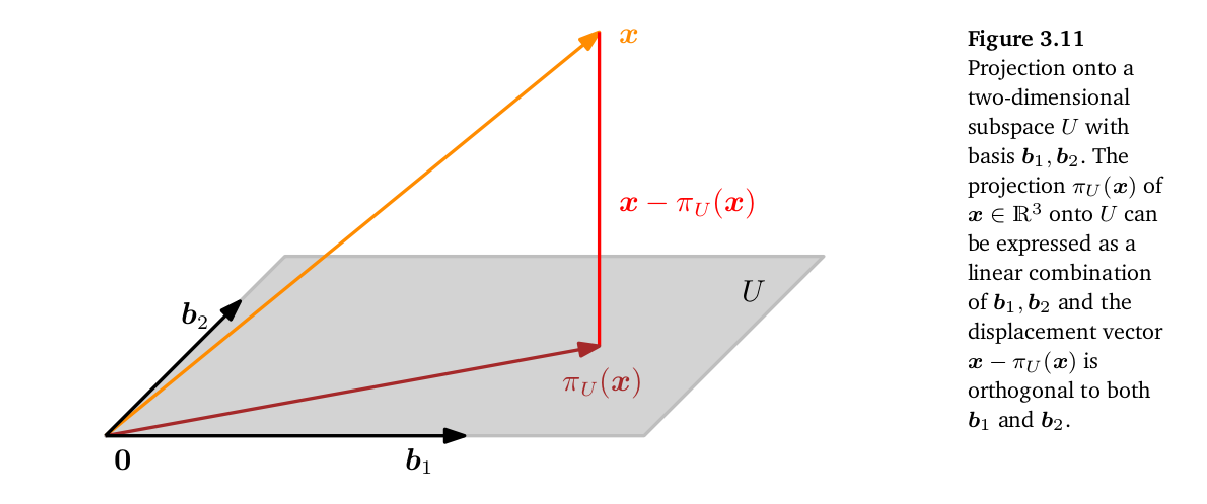
\includegraphics[width=0.95\textwidth,height=0.78\textheight,keepaspectratio]{figures/notes-md/N-20260305/N-20260305-fig-01-projection-onto-two-dimensional-subspace.png}
\caption{Projection onto a two-dimensional subspace: the residual \(x-\pi_U(x)\) is orthogonal to the basis directions of \(U\).}
\end{figure}

\section{Bridge to later ideas}

Projection is the geometric heart of least squares: the best approximation is characterized not by making the error small in every coordinate, but by making the error orthogonal to every allowed correction direction.



\paragraph{Expanded synthesis.}
For this chapter, the elementary material should be read as a study of what remains invariant when coordinates change. The earlier sections (`Projection onto a subspace`, `Projection matrix and least squares`, `Pseudoinverse`, `Higher viewpoint`) compute with arrays, bases, pivots, determinants, or eigenvectors; the deeper object is a linear map together with the spaces it acts on. A matrix is a representation of that map after bases have been chosen. This is why formulas such as
\[
  A' = P^{-1}AP,\qquad \widetilde A = T^{-1}AS
\]
are not cosmetic: they distinguish an intrinsic morphism from a coordinate description.

The structural hierarchy is as follows. Kernels record what a map forgets, images record what it reaches, cokernels record obstructions to solvability, and quotients record information after an equivalence has been imposed. Determinants act on the top exterior power and therefore measure oriented volume; traces are invariant under cyclic rearrangement and become characters in representation theory; adjoints depend on an inner product and lead to self-adjoint spectral theory.

A useful way to return to the computations is to ask, for every formula, which invariant it is measuring. Row reduction measures rank and kernel; diagonalization measures decomposition into invariant subspaces; Gram--Schmidt measures orthogonal projection; positive definiteness measures ellipsoid geometry; tensor notation measures how components transform. The elementary methods are therefore the finite-dimensional laboratory in which duality, quotienting, functoriality, and spectral decomposition can be seen clearly.


\section{Expanded derivation of the normal equations}

The formula for projection should not be memorized before the geometry is clear.  We want $B\lambda$ to be the closest vector in the column space of $B$ to $x$.  This means the error
\[
  e=x-B\lambda
\]
should be perpendicular to every vector in that column space.  Since the columns of $B$ span the space, this is equivalent to
\[
  B^T(x-B\lambda)=0.
\]
Hence
\[
  B^TB\lambda=B^Tx.
\]
If the columns of $B$ are independent, then $B^TB$ is positive definite and invertible.

\section{Four fundamental subspaces}

Projection is also a doorway to the four-subspace picture.  For a matrix $A$, the column space and left null space are orthogonal complements in the output space:
\[
  \mathbb R^m=\operatorname{Col}(A)\oplus \operatorname{Null}(A^T).
\]
Least squares solves $Ax\approx b$ by replacing $b$ with its projection onto $\operatorname{Col}(A)$.  The residual lies in $\operatorname{Null}(A^T)$.

\section{Pseudoinverse and minimum-norm solutions}

When $A$ is not full column rank, there may be many least-squares solutions.  The Moore--Penrose pseudoinverse selects the one with minimum norm.  Through SVD,
\[
  A=U\Sigma V^T,\qquad A^+=V\Sigma^+U^T.
\]
Small singular values are precisely the directions where inverse problems become unstable.
